%  !TeX  root  =  user_guide.tex

\chapter{QGIS Server}\label{label_qgisserver}
\index{WMS!QGIS Server}

% when the revision of a section has been finalized,
% comment out the following line:
% \updatedisclaimer

QGIS Server è un'implementazione WMS 1.3 open source con caratteristiche
molto avanzate per la produzione di carte tematiche.
QGIS Server è un'applicazione FastCGI/CGI (Common Gateway Interface) scritta 
in C++ e lavora in accoppiata ad un server web (es. Apache, Lighttpd). 
QGIS Server è supportato dai progetti europei Orchestra e Sany e dalla città 
di Uster in Svizzera.

A differenza di altri server WMS, QGIS Server usa come linguaggio di configurazione, 
sia per la configurazione a livello server che per le configurazioni utente, 
regole cartografiche in SLD/SE (Styled Layer Descriptor/Symbology Encoding)\footnote{\url{http://www.opengeospatial.org/standards/sld} e \url{http://www.opengeospatial.org/standards/symbol}}.
 
Sono, inoltre, disponibili plugin che permettono di esportare un progetto di 
QGIS desktop in un progetto web per QGIS Server, con regole di visualizzazione 
cartografica espresse in SLD. Dato che QGIS desktop e QGIS Server usano le stesse librerie, 
le mappe pubblicate sul web hanno la stessa visualizzazione di quelle in locale.
Per visualizzazioni cartografiche più complesse, è necessario configurare le regole
manualmente secondo le specifiche dello standard SLD e sue estensioni.

Si raccomanda la lettura del materiale ai seguenti indirizzi web:

\begin{itemize}
\item \url{http://karlinapp.ethz.ch/qgis\_wms/} \\
\item \url{http://www.qgis.org/wiki/QGIS\_mapserver\_tutorial} \\
\item \url{http://linfiniti.com/2010/08/qgis-mapserver-a-wms-server-for-the-masses/}
\end{itemize}

\section{Installazione di esempio su Debian Squeeze}

Di seguito è brevemente descritta un'installazione di esempio su Debian Squeeze. 
Anche molti altri OS hanno pacchetti precompilati per QGIS Server. Se si ha necessità 
di compilare da codice sorgente, riferirsi agli indirizzi web appena citati.

Oltre a qgis e qgis-mapserver, è necessario avere installato un server web, come ad esempio apache2. 
È possibile installare tutti i pacchetti necessari, e relative dipendenze, con aptitude o apt-get install.

Dopo l'installazione bisogna verificare il corretto funzionamento del server web e di qgis server. 
Assicurarsi che apache sia stato avviato con '/etc/init.d/apache2 start', aprire un browser ed andare su 
URL: http://localhost: se tutto è correttamente configurato dovrebbe apparire il messaggio 'It works!'.
Passare, quindi, a testare l'installazione di QGIS server

/usr/lib/cgi-bin/qgis\_mapserv.fcgi fornisce un WMS standard 
con visualizzati i confini degli stati degli USA \ref{fig:usa_wms}: caricare il WMS in QGIS con 
l'URL http://localhost/cgi-bin/qgis\_mapserv.fcgi, così come descritto nella Sezione \ref{sec:ogc-wms-servers}.

\begin{figure}[ht]
\centering
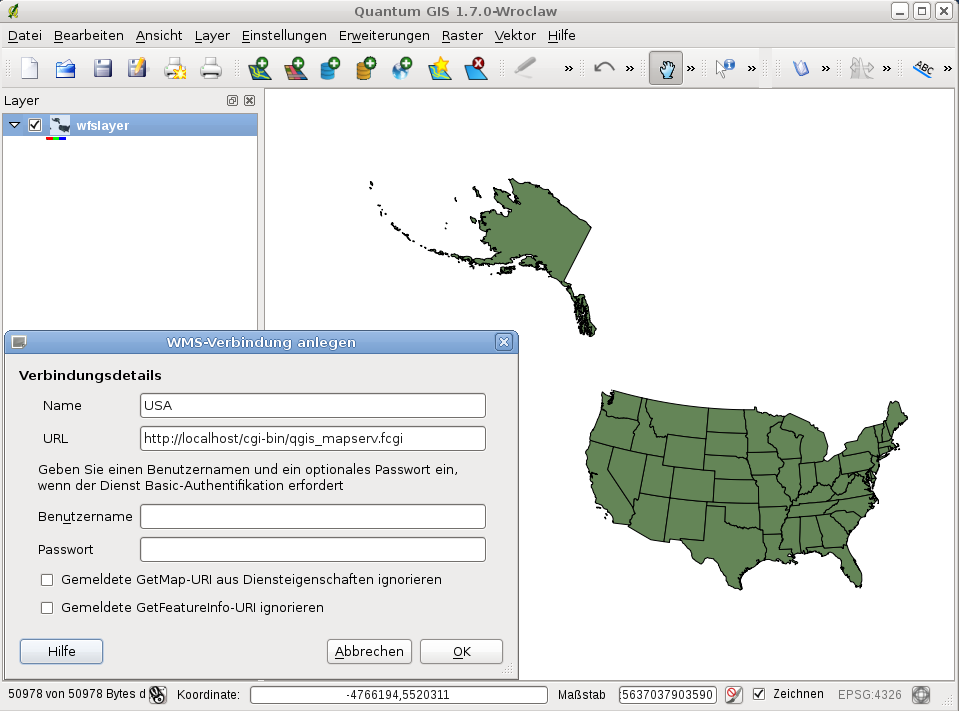
\includegraphics[clip=true, width=9cm]{standard_wms_usa}
\caption{WMS con i confini degli USA \nixcaption}
\label{fig:usa_wms}
\end{figure}

\section{Creare un WMS da un progetto QGIS}

Per offrire un servizio WMS si parte dalla creazione di un progetto QGIS: come esempio 
verranno utilizzati gli shapefile 'regions' e 'airport' da qgis\_sample\_dataset. 

\begin{itemize}[label=--]
\item Caricare in QGIS gli shapefile e definirne colori, stili e SR
\item Aprire la scheda \tab{WMS Server} sotto \mainmenuopt{Impostazioni} \arrow \mainmenuopt{Proprietà progetto...}
\item Attivare le caselle di controllo \checkbox{Service Capabilities} \checkbox{Estensione pubblicata} 
 \checkbox{Restrizioni dei sistemi di coordinate} e compilarne tutti i campi
\item Attivare la casella di controllo \checkbox{Aggiungi geometria WKT alle informazioni di risposta dell'oggetto}, 
se si vuole rendere il layer interrogabile
\item (Figure \ref{fig:wmsdefinition})
\item Salvare la sessione nel file di progetto 'alaska\_airports.qgs'.
\end{itemize}

\begin{figure}[ht]
\centering
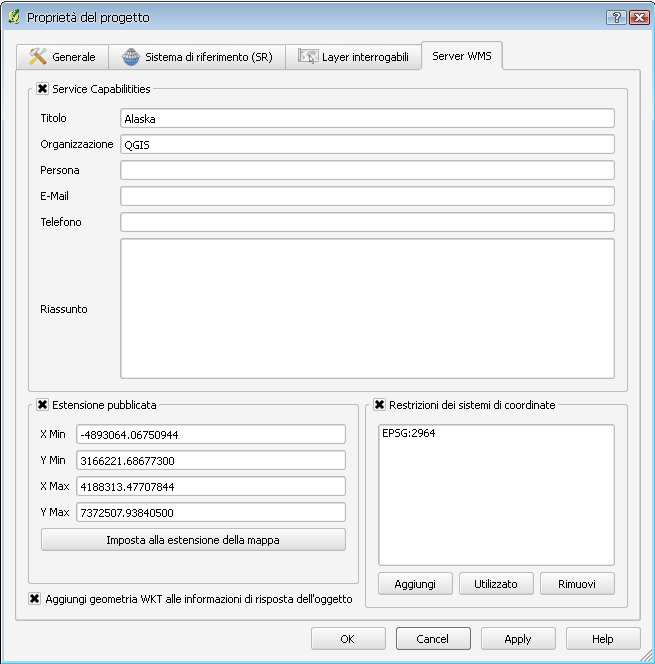
\includegraphics[clip=true, width=9cm]{wms_server_definition}
\caption{Definizione di un server WMS da un progetto di QGIS \wincaption}
\label{fig:wmsdefinition}
\end{figure}

Per fornire il progetto come WMS, creare una nuova cartella con diritti di amministratore '/usr/lib/cgi-bin/project' e 
copiarvi all'interno i file 'alaska\_airports.qgs' qgis\_mapserv.fcgi file.
Ora per testare il servizio, caricare il WMS in QGIS con l'URL http://localhost/cgi-bin/project/qgis\_mapserv.fcgi, 
così come descritto nella Sezione \ref{sec:ogc-wms-servers}: il risultato è mostrato in Figura \ref{fig:wmsproject}.

\begin{figure}[ht]
\centering
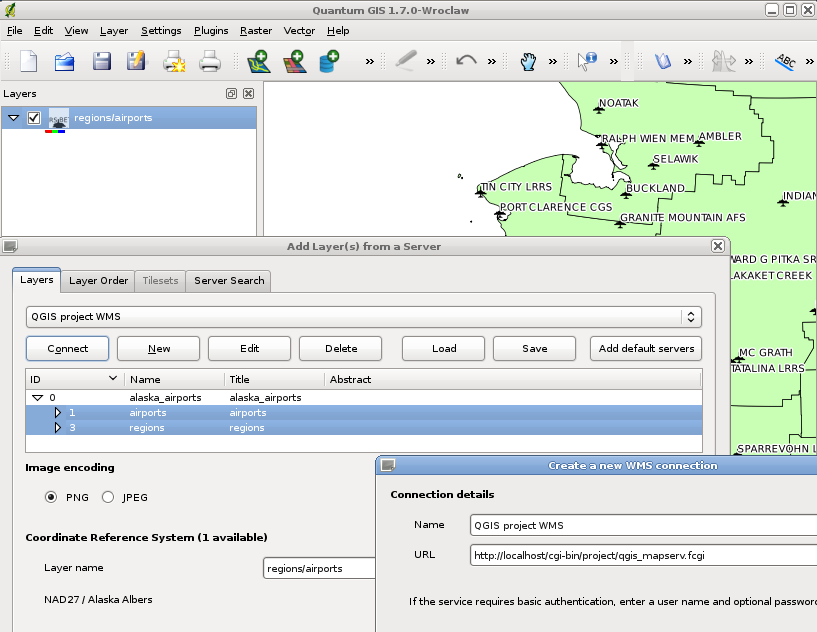
\includegraphics[clip=true, width=\textwidth]{wms_server_project}
\caption{Un server WMS basato su un progetto qgis \nixcaption}
\label{fig:wmsproject}
\end{figure}

\FloatBarrier
